\chapter{Using Tabling in \ourprolog} \label{tabling_overview}
%=============================================================
In addition to Prolog's SLD resolution, XSB has the ability to use SLG
resolution, which uses a type of {\em tabling}.  The difference in
evaluation strategy means that, with appropriate declarations, XSB is
complete under the well-founded semantics \cite{VGRS91} for
non-floundering normal programs (those with negation), and terminates
when these programs have the bounded term-depth property, as will be
explained below.  This use of tabling allows a different, more
declarative programming style than Prolog that can be of use for a
number of problems.  The following sections provide a brief
introduction to SLG resolution as it is implemented in XSB.  For
interested users, the ftp directory and web site contain papers
covering in detail various aspects of tabling.  An overview of SLG
resolution, and a practical evaluation strategy for it are provided in
\cite{ChWa96,SaSW95a,FSW98}. \cite{SaSw98,RRSSW98,JFLP-Scheduling,ChSW95}
describe fully the SLG-WAM as it is implemented in \version and
analyze its performance.

\section{SLG Evaluation}
%==============================

\subsection{Tabling}	
Consider the Prolog program
\begin{center}
\begin{minipage}{3.8in}
\begin{verbatim}
ancestor(X,Y) :- parent(X,Y).
ancestor(X,Y) :- ancestor(X,Z), parent(Z,Y).
\end{verbatim}						       
\end{minipage}
\end{center}
together with the query {\tt ?-ancestor(1,Y)}.  This program has a
simple, declarative meaning: {\tt Y} is an ancestor of {\tt X} if {\tt
Y} is a parent of {\tt X} or if {\tt Y} is a parent of an ancestor of
{\tt X}.  Prolog, however cannot compute the answer to this query.  It
enters an infinite loop.  The inability of Prolog to answer such
queries, which arise frequently, comprises one of its major
limitations as an implementation of logic.

A number of approaches have been developed to solve programs like
ancestor by reusing partial answers to the query {\tt ancestor(1,Y)}
\cite{Diet87,TaSa86,BMSU86,Viei89,Walk93}. Briefly, the ideas behind
these algorithms can be described in the following manner.  First, the
program keeps track of places where calls to {\tt ancestor(1,Y)} have
been made.  By maintaining this information, the repeated call to {\tt
ancestor(1,Y)} in the body of the second clause can be detected.  The
next idea is to store partial solutions to the call in a {\em table},
which consists of calls associated with their answers.  These answers
are substituted into the call to {\tt ancestor(1,Y)} in the body of
the second clause.  Once they are joined to the second literal of the
second clause these substitutions will in general produce new
solutions to the query, and these new solutions in their turn are fed
into the body of the second clause until a fixpoint (if any) is
reached.  In the language of
\cite{ChWa96}, the first call of a (leftmost) goal is called a
$generator$ node, and is expanded using program clauses as in SLD
resolution (Prolog).  Correct answer substitutions to the solution
node are interned in the {\em table entry} (call plus returns) for a
call.  Subsequent calls (that is, subsequent variant or subsumed
calls) are referred to as $active$ nodes
%
\footnote{Sometimes the term {\em consuming} nodes is also used in
this case.}, 
%
and are expanded using answers derived for that goal instead of
program clauses.  The computation ends when all possible program
clauses have been used to expand all $generator$ nodes, and when all
answers have been returned to all $active$ nodes.

Because $active$ nodes are expanded using answers rather than program
clauses, tabling will terminate whenever the set of answers to all
queries in a derivation is finite -- a situation which occurs when the
program has a finite model, for instance.  Indeed, it can be proven
that for any program with the {\em bounded term depth property} where
all terms have a maximum depth, SLG computation will terminate.  These
programs include the important class of {\em Datalog} programs.

It is important to notice two differences between tabling and SLD
resolution beyond termination properties.  First, termination requires
that each solution to a call be returned only once.  Second, because
of the way that solutions are stored and returned to $active$ nodes in
XSB, answers may be returned to the user in an unaccustomed order.

In XSB, predicates are executed Prolog style by default, and execute
by SLG resolution only if they are declared as tabled at compile time
using declarations like
\begin{center}
{\tt :- table(<Predicate>/<Arity>).}
\end{center}
The user can either make these declarations explicitly, or can get the
system to make them using the {\tt auto\_table} directive (see
Section~\ref{tabling_directives}).

The SLG-WAM overhead for SLD resolution is minimal.  Thus when XSB is
used simply as a Prolog system (i.e., no tabling is used), it is
reasonably competitive with other Prolog implementations based on a
WAM emulator written in C or assembly.  For example, XSB Version 1.6
is about two to three times slower than Quintus 3.1.1 or emulated
SICStus Prolog 3.1.

The bottom-up aspect of tabling in SLG aids in filtering out redundant
computations -- indeed it is this property which makes SLG complete
for non-floundering Datalog programs.  The same generation program
furnishes a case of the usefulness of tabling for optimizing a Prolog
program.
%---------------------------------------------------------------------()
\begin{example} \label{ex:same-gen} {\rm
The query {\tt ?- sg(1,X),fail.}\ was executed against the program
\begin{center}
\begin{Prog}
    sg(X,Y) :- cyl(X,X1), sg(X1,Y1), cyl(Y,Y1).	\\
    sg(X,X).
\end{Prog}
\end{center}
using a 24x24x2 randomly generated cylinder~\cite{BaRa86}, as the base
relation {\tt cyl/2}.  A cylinder can be thought of as a rectangular
matrix of elements where each element in row $N$ has links to a
certain number of elements in row $N+1$.  The 24x24x2 cylinder then,
is an array of 24x24 nodes, where each of the nodes in each row
(except the last) is connected to two elements in the next higher row.
Executing this query under SLG is more than three orders of magnitude
faster than under SLD, since SLD will search a complete binary tree of
depth 24.  }
\end{example}
%---------------------------------------------------------------------()

Tabling can generally be useful for optimizing data-orieted queries.
Section \ref{tabling_directives} illustrates how the {\tt
suppl\_table} directive can be used to aid in optimizing such queries.

While the judicious use of tabling can make some programs faster, its 
indiscriminate use can make other programs slower.  Naively tabling 
{\tt append/3} is one case
\begin{center}
\begin{minipage}{3.5in}
\begin{verbatim}
append([],L,L).
append([H|T],L,[H|T1]) :- append(T,L,T1).
\end{verbatim}						       
\end{minipage}
\end{center}
can, in the worst case, copy $N$ sublists of the first and third
arguments into the table, transforming a linear algorithm into a
quadratic one.

A non-trivial program that uses tabling can be found as part of the
XSB compiler, in \verb|$XSB_DIR/cmplib/mode.P|.

\section{Left-to-Right Dynamically Stratified Negation}
\index{negation!stratified}

Most of the original definitions for tabling algorithms considered
only definite programs, though some (e.g. \cite{KeTo88,Seki89})
extended tabling to programs with restricted forms of {\em stratified}
negation.  Broadly, a program uses stratified negation whenever there
is no recursion through negation.  Refining this intuition can lead to
an array of stratification classes.  While XSB evaluates all programs,
whether stratified or not, its evaluation is especially efficient for
\LRD\ programs \cite{SaSW95a}, which we now explain.

Consider a simple approach to incorporating negation into tabling, and
assume, to avoid complications of floundering, that the entire program
is ground --- that no clause of the program contains any variable.
Then if all predicates for negative literals are tabled, we could
evaluate a query to a program like
\begin{center}
\begin{minipage}{1.5in}
\begin{verbatim}
m :- c,a.
c :- b.
c.
b :- c,d.
a :- ~b.
\end{verbatim}
\end{minipage}
\end{center}
in a simple manner. Each time a negative goal is called, a separate
table is opened for the negative call.  This evaluation is carried on
to termination.  If it terminates, as it will for the classes of
programs in the last paragraph, its answers if any, are used to
determine the success of failure of the calling goal. 

The method just sketched is correct for certain classes of stratified
programs, but is not terribly efficient.  Every time a new negative
goal is called, a new table must be started, and run to completion.
We would like to use information already derived from the computation
to answer a new query, if at all possible.

XSB addresses this problem by keeping track of the {\em state} of each
call in the program table.  A call can have a state of {\em
not\_yet\_called}, {\em incomplete}, or {\em complete}.  The value
$not\_yet\_called$ means that there is in fact no table entry.  Calls
that do have table entries may be either $complete$ or $incomplete$.
A call is $complete$ only when its table entry contains all possible
solutions that are implied by the program, otherwise the call is
$incomplete$
%
\footnote{This use of completion allows ground queries to
Datalog programs with negation to be computed with polynomial data
complexity.}.
%
The scheduling strategy of program clause expansions and answer
returns in XSB allows for efficient detection of when a call may be
marked $complete$.

Using these concepts, we can now explain \LRD\ negation.  Assume we
have a tabled evaluation like that described in the previous
subsection: given a subgoal $S$ the evaluation uses information from
all clauses of $A$ and those which $S$ calls to solve $S$.  However,
literals within each clause are searched in a fixed left-to-right
traversal as in Prolog.  When a derivation path encounters a negative
literal, say $\neg L$, the behavior of the evaluation varies depending
on the state of $L$.  If $L$ is completed or has an answer, then
depending on its truth value, the path either fails or $\neg L$ is
removed from the list of subgoals to be resolved.  Otherwise the path
is {\em suspended}.  If $L$ has not yet been called, the evaluation
calls it; otherwise, if $L$ is incomplete (with no answers) the
evaluation proceeds to other clauses that may help determine the truth
of $L$.  If an answer is later found for $L$, the suspended derivation
path is failed, while if $L$ is determined to be completely evaluated
with no answers, $\neg L$ is removed from the derivation path which
then resumes its computation.

If a program $P$ can be evaluated using the method sketched above it
is called \LRD\ stratified.  The adjective ``left-to-right'' comes
from the fixed order in which the evaluation selects literals in the
body.  The adjective ``dynamic'' arises from the fact that run-time
information is central to whether the derivation path remains
suspended or not.  \LRD\ programs and their evaluation method are
explained in detail in \cite{SaSW95a,Przy89d}.  However, the following
simple program is \LRD, but does not fit into other stratification
classes (e.g. the more familiar class of {\em (left-to-right)
modularly stratified programs}~\cite{Ross91}.
\begin{center}
\begin{Prog}
p:- q,$\neg$ r,$\neg$ s.\\
q:-r,$\neg$ p. \\ 
r:-p,$\neg$ q. \\
s:-$\neg$ p,$\neg$ q,$\neg$ r. \\
\end{Prog} 
\end{center}

Before leaving the subject of stratification, we note that the use of
completion also forms the basis of evaluation of programs with
stratified {\tt findall/3} (See the description of predicate {\tt
tfindall/3} on page~\pageref{tfindall/3}).

\subsection{Dynamic Stratification}

A simple rearrangement of the program of the previous section causes
it not to be \LRD.  Consider the program
\begin{center}
\begin{Prog}
p:- $\neg$ s,,$\neg$ r, q.\\
q:-r,$\neg$ p. \\ 
r:-p,$\neg$ q. \\
s:-$\neg$ p,$\neg$ q,$\neg$ r. \\
\end{Prog}   
\end{center}
which cannot be evaluated by the method sketched above.  Such
programs, are called {\em dynamically stratified}, but may not be
stratified for any particular evaluation order \cite{Przy89d}.

\version\ of XSB handles dynamically stratified programs through
delaying negative literals when it becomes necessary to look to their
right in a clause, and then simplifying away the delayed literals when
and if their truth value becomes known.  However, to ensure
efficiency, literals are never delayed unless the engine determines
them to not to be stratified under the \LRD\ evaluation method.

\subsection{Non-Stratified Negation}
\index{negation!well-founded}

Russell's paradox, presented in Chapter 1, illustrates that when
negation appears in a logic program, recourse to a {\em three-valued
logic} may be necessary to describe its semantics.  That is, the value
of a ground atom may be {\em undefined} in addition to being true or
false.  From the perspective of stratification, these programs are not
even dynamically stratified.  XSB, in fact, handles such programs,
evaluating them according to the Well-Founded Semantics \cite{VGRS91}.
This semantics is a natural extension from a programmer's perspetive.
It can be shown that a program is dynamically stratified if and only
if it has a two-valued well-founded model.  Furthermore, more
elaborate forms of non-monotonic reasoning, such as stable models
\cite{GeLi88} can be built using the well-founded model.  Indeed, XSB
provides a residual program which, as explained below, can be used to
evaluate stable models of a program.

The intuition behind the Well-Founded semantics can be explained
through the operations of tabling.  First, consider how tabling acts
on a ground definite program.  Any ground atom is true if there is a
successful derivation of that atom, and false if every derivation path
ends in one of two cases.  In the first case, the path ends in a node
with a selected {\em generator} literal and there is no program clause
that can resolve the literal away.  In the second, the path ends in a
node with a selected {\em active} literal and there is no answer
clause which can resolve the literal away.  If all paths are failed by
the first case, the goal is said to be finitely failed, and the goal
would be failed by Prolog as well.  If any paths were failed through
the second case, it is possible that there would be infinite loops in
the Prolog derivation, and that Prolog would not fail the literal
properly.

In a definite program, the action of failing infinite recursion makes
intuitive sense.  In a normal program, though, recursion can occur
through negation, so that simply failing such recursion is
inappropriate.  For instance, if recursion through negation were
failed, the atom
\begin{Prog}
p:-$\neg$p.
\end{Prog}
{\tt p} would fail.  But then {\tt p} would be in any model of the
program making {\tt p} both true and false.  Assigning {\tt p} to be
both true and false makes the program inconsistent (among other
problems) so that reasoning in any program which has the above rule
becomes difficult at best.

The Well-founded semantics can be seen as an extension of dynamic
stratification to handle recursion through negation.  First, if an
atom, $A$, has a successful derivation, $A$ is true in the
well-founded model.  (With stratified negation, the notion of a
successful derivation may involve the full evaluation of negative
literals along with their completion, but remains intuitively clear).
If every clause defining $A$ fails (perhaps by delaying and checking
all literals in the clause) $A$ is false.  If neither of these cases
occur $A$ is undefined.  Thus $A$ is undefined if there is no
successful derivation of it and it is not failed through finite
failure or infinite positive recutsion.  That is, $A$ is failed if
after removing all successful literals in clauses that define $A$, and
after failing all clauses for $A$ with failed literals, recursion
through negation remains.

Many non-monotonic formalisms can be embedded into WFS, for instance
the Well-founded semantics with explicit negation, (WFSX)
\cite{ADP95}, adds explicit (or provable) negation to the default
negation used by the Well-founded semantics.  Using WFSX, problems in
domains such as diagnosis and hierarchical reasoning, or domains that
require updates \cite{Leit97}, can be easily modelled as logic
programs, and using the XSB preprocessor for WFSX (Section
\ref{library_utilities:wfsx}) such programs can be computed
efficiently.

\index{negation!stable models}
As a final point, \version\ of XSB also provides a basis for computing
stable models of a program through what is called the residual
program. Consider the simple, non-stratified program 
\begin{center}
\begin{Prog}
p:-$\neg$q,r. \\
q:-s. \\
q:-$\neg$p. \\
r. \\
\end{Prog}
\end{center}
there are two stable models of this program: on in which {\tt p} and
{\tt r} are true, and another in which {\tt q}, and {\tt r} are true.
In the Well-Founded model, {\tt r} is true, {\tt s} is false, and {\tt
q} and {\tt p} are undefined.  As mentioned above, SLG delays literals
whose truth value cannot be determined and later simplifies the
delayed literals away when and if their truth value becomes known.
Those delayed literals which are not simplified away, therefore, may
either be true or false in a given stable model of a program, and the
computation of the Well-Founded model performed by XSB can be seen as
a pre-processor for stable models.  The pre-processed program consists
of all answers whether they have a delay list (are {\em conditional})
or not (are {\em unconditional}).  This program is called the {\em
residual program}, and in such a program delayed literals are treated
as body literals of a clause.  The residual program for the above
program would be. 
\begin{center}
\begin{Prog}
p:-$\neg$q. \\
q:-$\neg$p. \\
r. \\
\end{Prog}
\end{center}
Computing stable models is an intractible problem.  The residual
program may have evaluated away clauses and body literals from the
original program.  For a ground program, if it is ensured that
residual clauses are produced for all atoms, using the residual
program may bring a performance gain since the search space of
algorithms to compute stable models will be correspondingly reduced.
In fact, by using XSB in conjunction with a Stable Model generator,
Smodels \cite{NiSi96}, an efficient system has been devised for model
checking of concurrent systems that is 10-20 times faster than
competing systems \cite{RaSm97}.


\section{Tabling in a Prolog Environment}\label{tabling_env}
%===========================================================

Four of the goals of XSB are 
\begin{itemize}
\item	To execute tabled predicates at the speed of compiled Prolog.
\item	To ensure that the speed of compiled Prolog is not slowed
	significantly by adding the option of tabling.
\item	To provide Prolog functionality in tabled predicates 
	whenever it is semantically sensible to do so.
\item	To provide standard predicates to manipulate tables
	taken as objects in themselves.
\end{itemize}

In order to accomplish the first two of these goals, the {\em Warren
Abstract Machine (WAM)} which serves as the engine of Prolog was
redesigned to allow tabling.  (The new engine is called the SLG-WAM).
While most WAM instructions were affected by the redesign, SLG-WAM
execution is only 10-20\% slower than a WAM execution on a similar
engine.  Beyond the comparison with Prolog, our implementation
strategy has several implications which may affect the user.

First, \ourprolog's evaluation is top-down, and solutions are derived
a tuple at a time.  This characterization allows it to be contrasted
with, say, magic sets~\cite{BMSU86} which evaluate queries
bottom-up and derive solutions a set at a time.  There are advantages
and disadvantages to \ourprolog's evaluation method.  One advantage is
that the top down derivation maintains a representation of the state
of a search, and because of this, answers are never returned to
improper goals, then filtered out, as can happen in a bottom-up
evaluation method.  Another is that, since tabling is done at the
SLG-WAM level, the engine is very efficient.  There are associated
disadvantages with our paradigm, though.  Firstly, we copy structures
between the execution stacks and table space, rather than allowing
sharing between the two spaces\footnote{It is possible to avoid
copying in the case of ground strucures, but this is not implemented
for the trie-based table structures of \version}.  Also, since
\ourprolog's evaluation is tuple-at-a-time, it is not particularly
efficient for queries to large relations which are kept on
disk\footnote{To address this problem, an alternate breadth-first
search strategy is under development the goal of which is to provide a
set-at-a-time search at the speed of the current tuple-at-a-time
engine.}.

Tabling integrates well with most Prolog functionality.  The use of
negation and aggregates in tabled predicates was discussed in the
precious section.  Other Prolog predicates, such as meta-logical
predicates like {\tt var/1}, predicates with side-effects like {\tt
read/1} and {\tt write/1} can be used freely in tabled predicates as
long as it is remembered that only the first call to a goal will
execute program clauses: the rest will look up answers from a table.
If the user wants to reexecute the program clauses for any reason, the
Prolog predicates {\tt abolish\_all\_tables/0, abolish\_table\_pred/1}
or {\tt abolish\_table\_call/1} can be used, which will cause new
calls to a goal to execute program clauses, in addition to removing
the information in tables.  Standard tabling predicates are described
in Section~\ref{tabling_predicates}

Cuts are allowed in tabled predicates, subject to the restriction that
the scope of a cut cannot include a call to a tabled predicate.  The
way this description works can be seen most easily from an example.
Suppose {\tt t/2} is a tabled predicate.  Then the definition
\begin{center}
\begin{minipage}{1.7in}
\begin{verbatim}
t(A,B) :-
      p(A,B), ! ...
t(A,B) :- 
      r(A,B), ...
\end{verbatim}						       
\end{minipage}
\end{center}
is allowed, but a body with
\begin{center}
\begin{minipage}{1.5in}
\begin{verbatim}
        :
        t(A,B),
        !,
        :
\end{verbatim}						       
\end{minipage}
\end{center}
is not allowed because the table corresponding to the call of {\tt
t(A,B)} will never be completed.  Furthermore, there can also be cuts
in the dependency graphs of {\tt p/2} and {\tt r/2}, subject to the
scope restriction.  The \ourprolog\ compiler checks for violation of
the scope restriction.

A similar situation occurs when the user makes a call to a tabled
predicate from the interpreter level, but does not generate all
solutions.  In such a case, the user will see the warning {\tt
"Removing incomplete tables..."} appear.  Any complete tables will
not be removed.  They can be abolished using one of the predicates
mentioned above.

As a final point, it is often useful to manipulate tables in a
non-logical way, for instance to create meta-interpreters.  To do so
we provide a number of standard predicates.  The user is provided with
the means to backtrack through all calls in a table, to backtrack
through all returns in a call, to find out the state of a given table,
to reset properties of given tables or to abolish them.

\section{Using different scheduling strategies in XSB}
%==============================
\index{Local Scheduling}

Given the asynchronicity of answer generation and answer return,
tabling systems face an important scheduling choice not present in
traditional top-down evaluation: How does the order of returning
answers to consuming subgoals affect program efficiency.  The
scheduling of answer returns is an important issue for effiency of
evaluations.  Indeed, the tabling scheduling strategy of XSB was
thoroughly revised in version 1.5 to use a strategy that is more
efficient in terms of time and space \cite{JFLP-Scheduling}.

The same paper outlined implementatoin of a second scheduling
strategy, \localsched, which has applications to non-monotonic
reasoning and when combined with answer subsumption can improve the
performance of some programs by arbitrary amounts. In \localsched\ the
engine evaluates a single dynamic SCC at a time --- preserving the SCC
ordering during the evaluation.  In other words, answers are returned
outside of an SCC (that is, to consuming nodes in trees whose root
subgoal is not in the SCC) only after that SCC is completely
evaluated.  The actions of \localsched\ can easily be seen through the
following example of stratified evaluation.

\begin{example} \label{ex:cascade-susps} \rm
Let \emph{P} be the modularly stratified program:
\begin{verbatim}
:- table a/0,b/0,c/0,d/0,e/0,g/0,h/0,i/0,j/0.

a:-b,c,d.     b:-e.         c:-h. 
              b:-g.         c:-i.
 
d:- tnot(h).  e:-b,s.       g.            

h:-j.         j:- tnot(e).  i.                             
\end{verbatim}
\noindent
for which the query {\tt ?- a} is to be evaluated.  If evaluated under
either \oldsched\ (XSB v.~1.4) or \newsched, an SDG will be produced
with cascading negative dependencies as shown in
Figure~\ref{fig:lrd-pgm}(a).  Even though there is no cycle through
negation, detecting this property can complicate the evaluation of
stratified programs. However if \localsched\ is used, a \emph{simpler}
SDG is created (as depicted in in Figure~\ref{fig:lrd-pgm}(b)). To attain
this latter SDG, each independent SCC has to be completely evaluated
before returning any answers to subgoals outside the SCC --- making the
search depth-first with respect to SCCs.  In \localsched, the SCCs {\tt
\{b, e\}} and {\tt \{g\}} are completely evaluated before {\tt b}
returns any answers to {\tt a}. Thus, {\tt e} is completely evaluated
when {\tt tnot(e)} is called and negative dependencies are not created.
The negative link from {\tt j} to {\tt e}, and that from {\tt d} to {\tt
h} are avoided, since both {\tt e} and {\tt h} are completed by the time
they are called negatively.

\begin{figure}[htb]
\centering
\mbox{\subfigure[Negative dependencies]{
\epsfig{file=cascaded.eps,height=4cm}}\quad
      \subfigure[No negative dependencies]{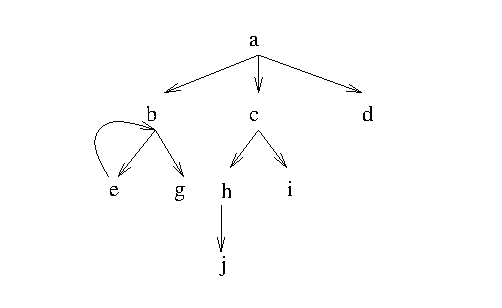
\epsfig{file=no-cascade.eps,height=4cm}}\quad
     }
\caption{\emph{Subgoal dependency graphs for program \emph{P} of
Example~\ref{ex:cascade-susps} under different search strategies}}
\label{fig:lrd-pgm}
\end{figure}

\end{example}

\Localsched\ can improve the performance of programs that benefit
from answer subsumption in the following manner.  Answer subsumption can
be performed as a variation of the SLG {\sc new answer} operation. While
adding an answer, the engine may check whether that answer is more
general than those currently in the table.  If it is more general, this
new answer is added and the subsumed answers are removed (otherwise, the
answer is simply discarded).  Given that \localsched\ evaluates each SCC
completely before returning any answers out of it, we are guaranteed
that only the most general answers will be returned out of that SCC.

\comment{
That would be nice, but will it happen?

In an upcoming release, XSB will allow \localsched\ to be defined at
the predicate level.
}
